\documentclass[a4paper,11pt]{article}
\usepackage{jinstpub}
\usepackage{lineno}
\usepackage[outdir=./]{epstopdf}
\usepackage{multicol}
\usepackage{multirow}
\usepackage{longtable}
\usepackage{array}
\usepackage{rotating}
\usepackage{arydshln}

\usepackage{ptdr-definitions}
\usepackage{custom-definitions}

\usepackage{enumerate}

\graphicspath{
{Figures/}
}

\newcommand{\orc}{
\includegraphics[height=\fontcharht\font`A]{orcidlogo}}
\newcommand{\orcid}[1]{\href{https://orcid.org/#1}{\orc}}
\newcommand{\kernum}[1]{\ensuremath{#1^\prime}\xspace}


\linenumbers


\title{Convolutional decoding of surface codes}

\author{Ula{\c s}can Sar{\i}ca\orcid{0000-0002-1557-4424}}
\affiliation{University of California, Santa Barbara\\Santa Barbara, CA, USA}

\emailAdd{ulascan.sarica@cern.ch}

\abstract{
}



\begin{document}
\maketitle
\flushbottom


\section{Kernel construction for convolutions}

\section{Translating kernel outputs as inputs to higher-order layers}

%%%%%%%%%%%%%%%%%%%%%%%%%%%%%
\begin{figure*}[htb]
\centering
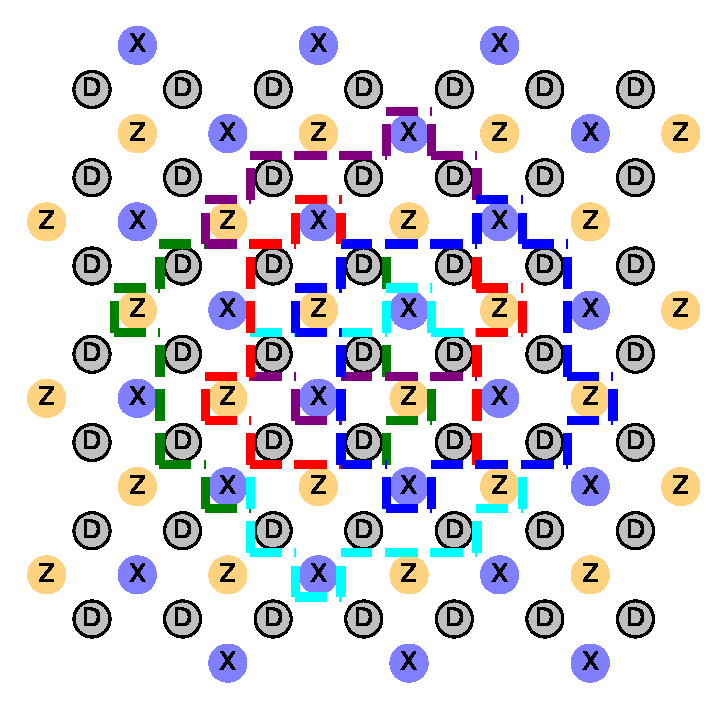
\includegraphics[width=0.6\textwidth]{d7_q25_kernels.pdf}
\ccaption
{$d=3$ kernels surrounding a data qubit in a $d=7$ surface code}
{
}
\label{fig:d7wkern}
\end{figure*}
%%%%%%%%%%%%%%%%%%%%%%%%%%%%%

In the example shown for a $d=7$ code in Fig.~\ref{fig:d7wkern}, all of the displayed kernels are of the same unique type. We highlight the central red kernel as a standard $d=3$ surface code patch and the blue one corresponding to its flipped counterpart. For simplicity, we will number all data qubits from 1 (top left) to 7 (top right) and 49 (bottom right). We will denote the corresponding qubit numbers on the kernel patch with a prime indicator, \eg, qubit 18 $\rightarrow$ \kernum{2} in the red kernel and \kernum{3} in the blue one.

As the kernels assume uniform noise to maximize the number of weights shared, only the weights that are associated with kernel qubits \kernum{1}, \kernum{2}, \kernum{3}, \kernum{5}, \kernum{6}, and \kernum{9} are unique. For that reason, these kernels have 6 outputs instead of 9, as it would be the case for kernels at the boundary.

The overlaps of red and blue kernels occur over qubits 18, 19, 25, 26, 32, and 33 (\kernum{2}, \kernum{3}, \kernum{5}, \kernum{6}, \kernum{8}, and \kernum{9} in the red kernel).





\end{document}
